
\chapter{基于简化社会力模型的混合交通仿真}
\label{chapter:simplified}

%在先前的工作中,研究者为了提高交通仿真可视化结果的真实性,已经考虑了诸如夜景或天气因素。然而在这些仿真器中,有的仅包含车辆这一单一种类的交通参与者,而有的则把行人和自行车等简单地视为按照预定义行为运动的个体,仅考虑车辆对这些个体做出的反应,缺乏不同种类个体之间的相互影响。因此,为了模拟更真实的城市级别混合交通场景,一个能综合考虑车辆、自行车和行人等多种类智能体之间交互行为的仿真器是十分具有价值的。

在先前的章节中,本文通过引入交互式仿真技术,提出了适配不同用户编辑交互操作的运动控制策略,从而将一系列非常规的驾驶行为引入了交通仿真中,这些行为利用现有的方法难以生成,数据集中出现的频率较低,但现实世界的交通中却会真实发生。虽然这些方法提高了仿真个体的运动多样性,但仅包含车辆这一单一种类的交通参与者,而真实交通中包含了大量机动车、非机动车、行人等不同种类个体的之间交互影响。因此,在一个统一的框架内模拟城市级别的混合交通场景,提升仿真个体的种类多样性,也是提升可视化交通仿真数据多样性的一个方向。


最近,Chao等人提出了一种基于社会力的混合交通仿真框架,首次将行人、车、自行车的行为和相互影响抽象为社会力表示并在统一的框架中实现~\cite{chao2019force}。对于某一个交通参与者来说,作用在其身上的力可以分为驱动其接近预期目标的驱动力,来自环境中障碍或标线的排斥力,以及不同类型智能体之间的相互作用力。然而,该框架为其包含的每一种智能体在混合交通环境中都定义了完全不同的运动控制策略,导致计算各类社会力所使用的模型,对不同种类智能体也各不相同,模型中涉及到的参数更是“专人专用”。这样的结构使得整个框架包含了大量需要预定义的参数,无形中增加了用户调试参数的成本;且诸多“缩放因子”或“敏感因子”只用于规范和缩放力计算表达式最终的输出数值,并无实际的物理意义,不利于用户直观感受到参数变化和智能体行为变化之间的联系——这些都与我们提升用户交互体验的初衷相违背。因此,这启发了我们提出一个简化的运动控制模型,在仅使用少量参数的情况下统一描述不同个体行为共性;同时,又能在不引入大量用户调试操作的情况下使模型泛化出不同种类智能体的个性化行为。


由于不同种类的智能体在行为模式上的差异巨大,想要构建一个简化的混合交通仿真框架并非易事,例如:在遵守交通规则的情况下,车辆必须沿着正确的车道行驶,而行人和自行车可以在其对应道路内更自由地运动;车辆和自行车的运动都严格遵守车辆运动学模型,而行人的运动则有更大的自由度可以瞬时改变速度朝向等等。综上所述,本章提出了一种基于简化社会力模型的混合交通仿真方法,旨在引入一个更简洁、更易扩展的框架来统一仿真不同种类智能体的行为和相互影响。图~\ref{fig:simplified_snapshot}展示了使用本方法仿真的包含行人、车、自行车的混合交通场景。具体来说,通过分析Chao等人的工作~\cite{chao2019force},我们发现其所使用的不同社会力模型本质上都具有相似的函数形式,且模型中包含的若干不具有实际物理意义的控制参数,可以使用智能体属性建模实时计算进行替代。所以,基于面向对象的思想,本方法首先设计了一个基类用于表达上述不同种类智能体之间行为的共性,并用一个简化的社会力模型去刻画个体间交互行为中沿着点到点方向的影响和垂直该方向的影响。为了将该基类派生为不同的个体,本方法使用不同种类的智能体的具体物理属性,例如速度、加速度、反应时间和跟随距离等,来参数化模型中的系数,减少了无实际物理意义参数的同时,也实现了混合交通参与者的多态性。本方法的主要贡献如下:

\begin{figure}[!t]
\centering
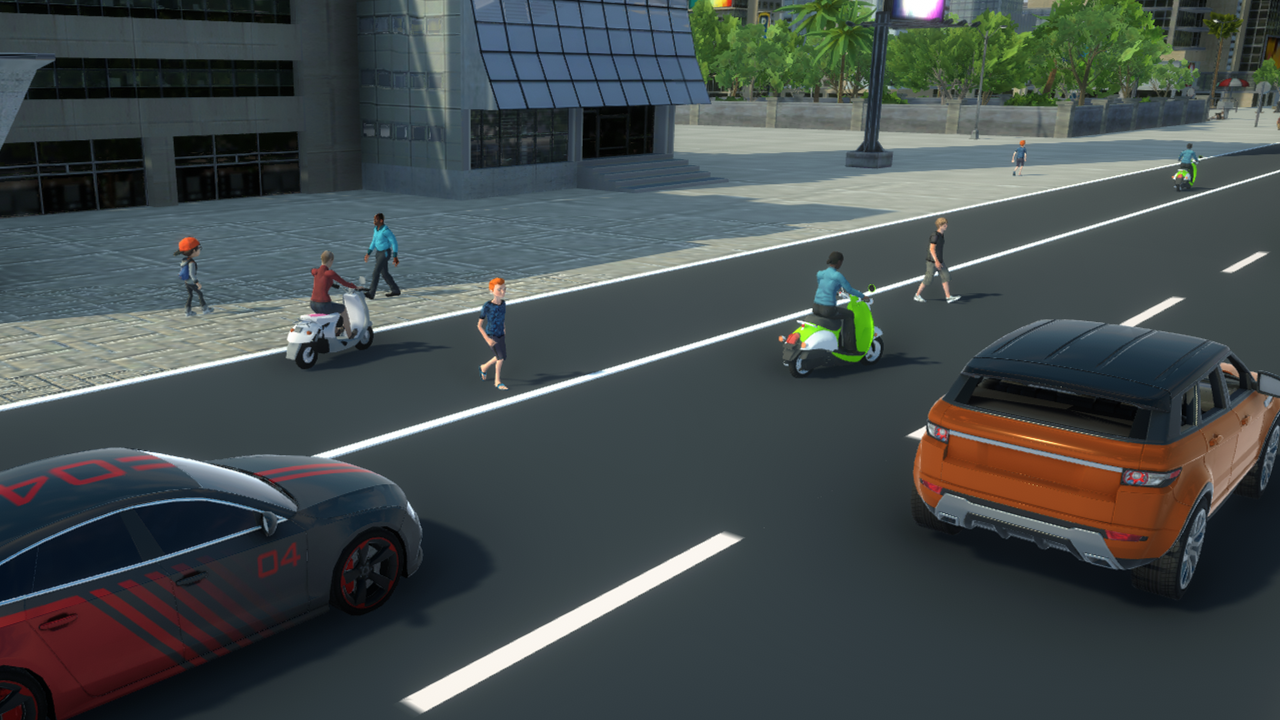
\includegraphics[width=0.8\textwidth]{figure/simplified/simplified_snapshot9.png}
%\caption[基于简化社会力模型仿真的混合交通场景]{
%基于简化社会力模型仿真的混合交通场景结果示意图。}
\caption[基于简化社会力模型仿真的混合交通场景]{
基于简化社会力模型仿真的混合交通场景
}
\label{fig:simplified_snapshot}
\end{figure}

\begin{itemize}
    %\item 基于面向对象的思想,设计了一个能描述不同种类智能体行为共性的基类。

    %\item 提出了一个简化的社会力模型,用于高效计算混合交通中不同个体间的相互影响。

    %\item 使用个体属性将模型系数参数化,从而派生出不同种类的智能体,并使得同类个体的行为多样化。

    \item 提出了一个简化的社会力模型,用于统一、高效地计算混合交通仿真中个体的运动和不同种类个体之间的相互影响。

    %\item 提出了一个混合交通仿真的框架,首先基于面向对象的思想设计了一个抽象的基类用于描述不同种类智能体运动的共性,然后利用个体参数对基类中的社会力模型参数化,进一步派生出不同种类的智能体。

    \item 基于面向对象中派生—多态的思想,设计了一个能在非欧坐标下表征不同个体运动共性的基类,并利用个体属性参数化基类中的社会力模型参数,进而派生出不同种类的个体。

    \item 基于提出的简化社会力模型与派生结构实现了包含人、车、非机动车的混合交通仿真,提高了仿真智能体种类多样新的同时,与先前的方法相比减少了大量的冗余参数,并在个体属性变化与行为变化之间建立了直观联系,避免用户进行繁琐的调参。
    
\end{itemize}





\section{方法概述}


图~\ref{fig:simplified_overview}展示了本方法的流程。通过对先前交通仿真中所使用的所有社会力模型进行分类分析(章节~\ref{section:simplified_decayfunc}),我们基于面向对象的思想定义了一个能统一描述智能体行为共性的基类,其中除了包括某一个体的目标对其施加的自驱动力,还用一个简化的社会力模型表示其与周围个体或环境交互时的交互力,该交互力可分解为沿着两智能体连线方向的直接排斥力和垂直该方向的横向避让力(章节~\ref{section:simplified_basicclass})。对于上述简化的社会力模型中的计算系数,我们使用每个个体的特有物理属性进行参数化,将基类派生为不同种类的智能体,最终得到包含行人、车、自行车的混合交通仿真结果(章节~\ref{section:simplified_parameterize})。在结果部分,我们展示了基于本方法仿真得到的混合交通中不同个体的交互案例(章节~\ref{section:simplified_interactioncase}),并验证了在性能方面本方法提出的简化社会力模型比先前的方法中所使用的社会力模型具有更高的计算效率(章节~\ref{section:simplified_performance})。

\begin{figure}[!htb]
\centering
%\setlength{\abovecaptionskip}{0.1cm}
%\setlength{\belowcaptionskip}{-0.2cm}
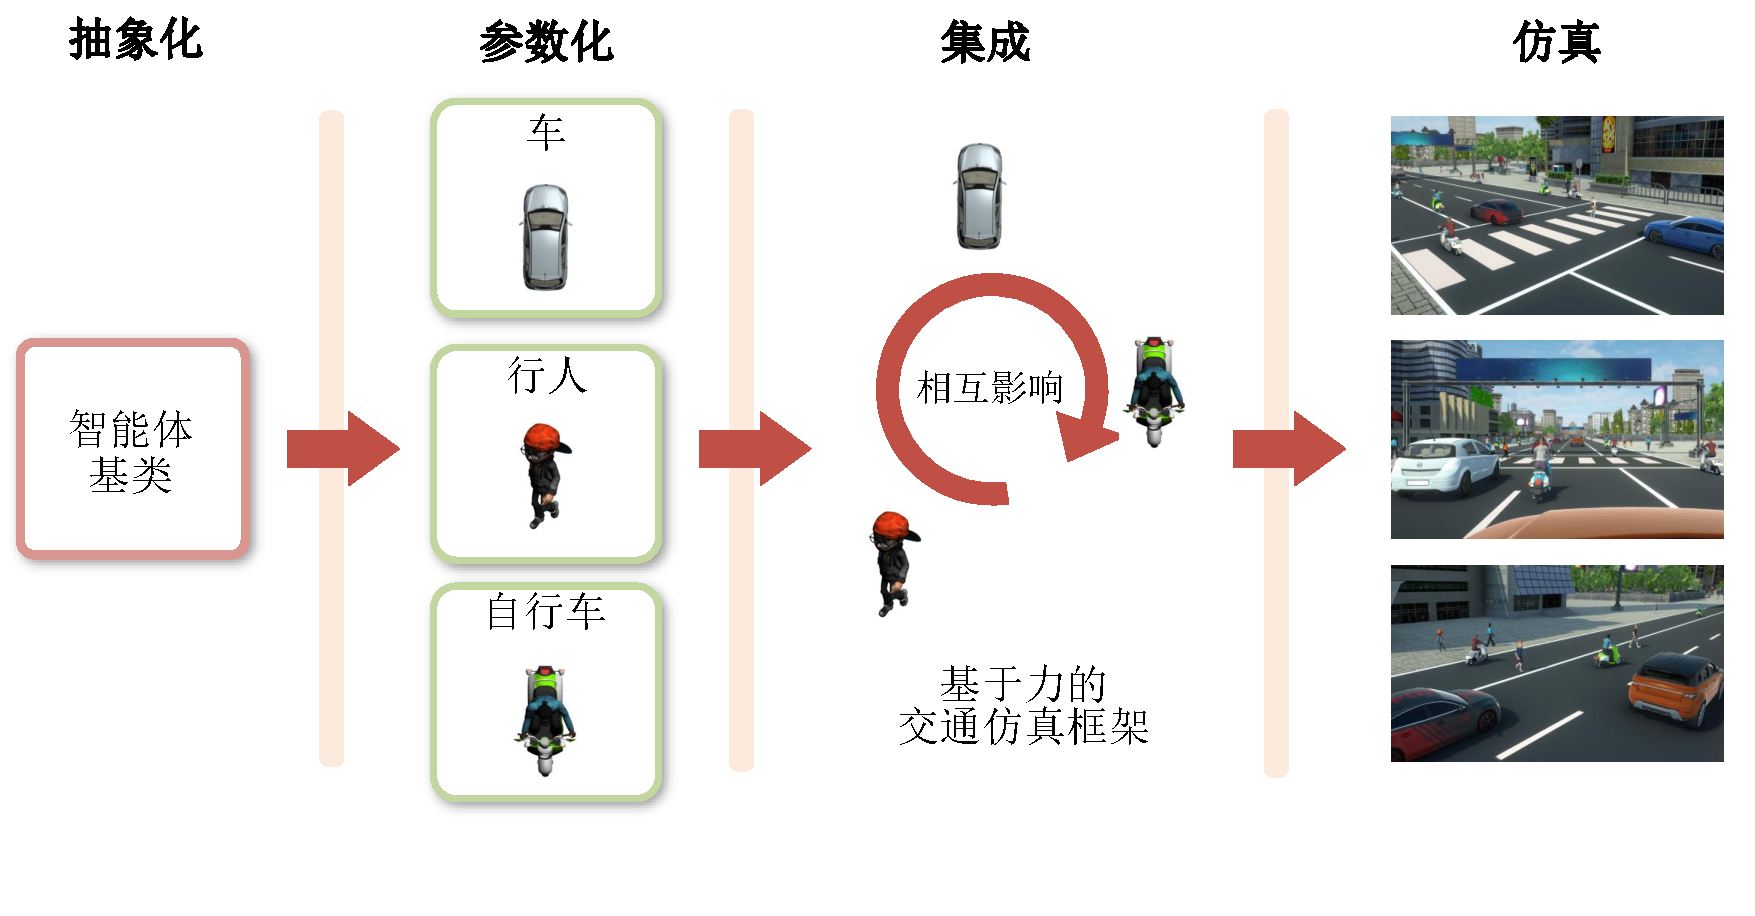
\includegraphics[width=\textwidth]{figure/simplified/simplified_overview_cn.pdf}
%\caption[基于简化社会力模型的混合交通仿真流程示意图]{
%基于简化社会力模型的混合交通仿真流程示意图。我们首先定义了一个能统一描述智能体行为共性的基类,然后基于个体的特有物理属性对系数进行参数化,将基类派生出不同种类的个体,最后集成到仿真框架中得到包含行人、车、自行车的混合交通仿真结果。}
\caption[基于简化社会力模型的混合交通仿真流程图]{
基于简化社会力模型的混合交通仿真流程图
}
\label{fig:simplified_overview}
\end{figure}


\section{指数衰减型力计算模型}
\label{section:simplified_decayfunc}


根据Chao等人的工作~\cite{chao2019force}的定义,对任意智能体$i$而言,其运动由目标、其他智能体和环境因素所施加的各个类型力的合力决定:
\begin{equation}
\setlength\abovedisplayskip{6pt}
\setlength\belowdisplayskip{6pt}
\label{eq:simplified_previous}
    \textbf{F}_i = \textbf{F}_i^0 + \sum_{j(\not=i)}\textbf{F}_{ij} + \sum_{o}\textbf{F}_{io} +  \sum_{W}\textbf{F}_{iW},
\end{equation}
其中,$\textbf{F}_i^0$表示智能体$i$的自驱动力驱使$i$以预期速度接近目标,$\textbf{F}_{ij}$表示同类型的邻近智能体$j$对$i$施加的交互力,$\textbf{F}_{io}$则表示不同类型的邻近智能体$o$对$i$施加的交互力,$\textbf{F}_{iW}$表示环境因素$W$对$i$施加的力,如车道线或障碍物等。


\begin{table}[!b]
%\setlength{\abovecaptionskip}{-0.2cm}
\setlength{\belowcaptionskip}{0.4cm}
%\begin{center}
\centering
%\caption[指数衰减函数分类与应用统计]{
%Chao等人的工作~\cite{chao2019force}中所使用的不同形式的指数衰减型函数,与它们所应用的交互行为的分类统计。}
\caption[Chao等人方法使用的社会力模型的统计与分类]{
Chao等人方法~\cite{chao2019force}使用的社会力模型的统计与分类
}

\label{tab:simplified_decayfunc}
\renewcommand\arraystretch{1.5}
\setlength{\tabcolsep}{10.3mm}{
\begin{tabular}{|c|l|}
\hline
\multicolumn{1}{|l|}{\textbf{函数基本形式}} & \textbf{应用于交互行为}  \\ \hline
$f(x)=e^{-x}$                            
& \begin{tabular}[c]{@{}l@{}}智能体 - 道路边界\\ 车 - 车 (邻车道)\\ 车 - 自行车 (侧方)\\ 自行车 - 自行车 \\ 自行车 - 车 (侧方)\\ 行人 - 行人 \end{tabular} \\ \hline
$f(x)=\frac{1}{x^2}$                
& \begin{tabular}[c]{@{}l@{}} 车 - 车 (同车道)\\ 车 - 行人 \\ 车 - 自行车 (前方)\\ 自行车 - 车 (前方) \end{tabular} \\ \hline
$f(x)=e^\frac{1}{x}-1$                           
& 自行车 - 行人 \\ \hline
$f(x)=x^{-0.67}$                        
& \begin{tabular}[c]{@{}l@{}} 行人 - 车 \\ 行人 - 自行车 \end{tabular} \\ \hline
\end{tabular}} 
\end{table}


对于智能体$i$的自驱力$\textbf{F}_i^0$,其由该智能体的质量$m_i$,预期行驶速度$\textbf{v}^{0}_{i}$和最大加速度$\textbf{a}_{i}$决定~\cite{helbing2000simulating}:
\begin{equation}
\label{eq:simplified_selfmotivation}
    \textbf{F}_i^0 = m_{i} \frac{\textbf{v}^{0}_{i} - \textbf{v}_{i}}{\textbf{v}^{0}_{i}} \textbf{a}_{i}.
\end{equation}
而对于各个类型智能体之间的交互行为,他们使用了一系列不同的函数模型来计算表达式~\ref{eq:simplified_previous}中的各类社会力。通过对这些力计算模型进行分类分析,我们发现其中总共包含四种基本的函数形式。我们将分类的结果和每种类型函数所应用于的交互行为列举在表~\ref{tab:simplified_decayfunc}中,并将函数图像展示在图~\ref{fig:simplified_decayfunc}(a)中。根据观察图像我们发现,所有基本类型的函数均具有指数衰减的趋势,即在区间$(0, +\infty)$内单调递减,当$x$趋近于$+\infty$时所有函数趋近于$0$,当$x$趋近于$0$时除函数$e^{-x}$趋近于$1$以外,其余函数均趋近于$+\infty$。假如将两个函数之间的差异定义为在给定区间内对应函数曲线围成的面积大小,我们可以通过为上述四种的指数衰减型函数添加特定的系数来平移或缩放函数曲线,从而减小他们之间的差异。如图~\ref{fig:simplified_decayfunc}(b)所示例子,我们将函数$e^{-x}$转变为$10e^{-2.2x}$,则在区间$(0.5, +\infty)$内其与函数$\frac{1}{x^2}$的差异只有:
\begin{equation}
\label{eq:simplified_funcdiff}
        \int_{0.5}^{+\infty} \left| \frac{1}{x^2} - 10e^{-2.2x} \right| dx \approx 0.60472.
\end{equation}
换言之,若以两智能体间的距离为变量,分别用这两个函数计算智能体间排斥力的大小,则在距离大于0.5个单位的时候,计算结果数值上至多只有0.60472的差异。



\begin{figure}[!tbh]
\centering
%\setlength{\abovecaptionskip}{0.1cm}
%\setlength{\belowcaptionskip}{-0.2cm}
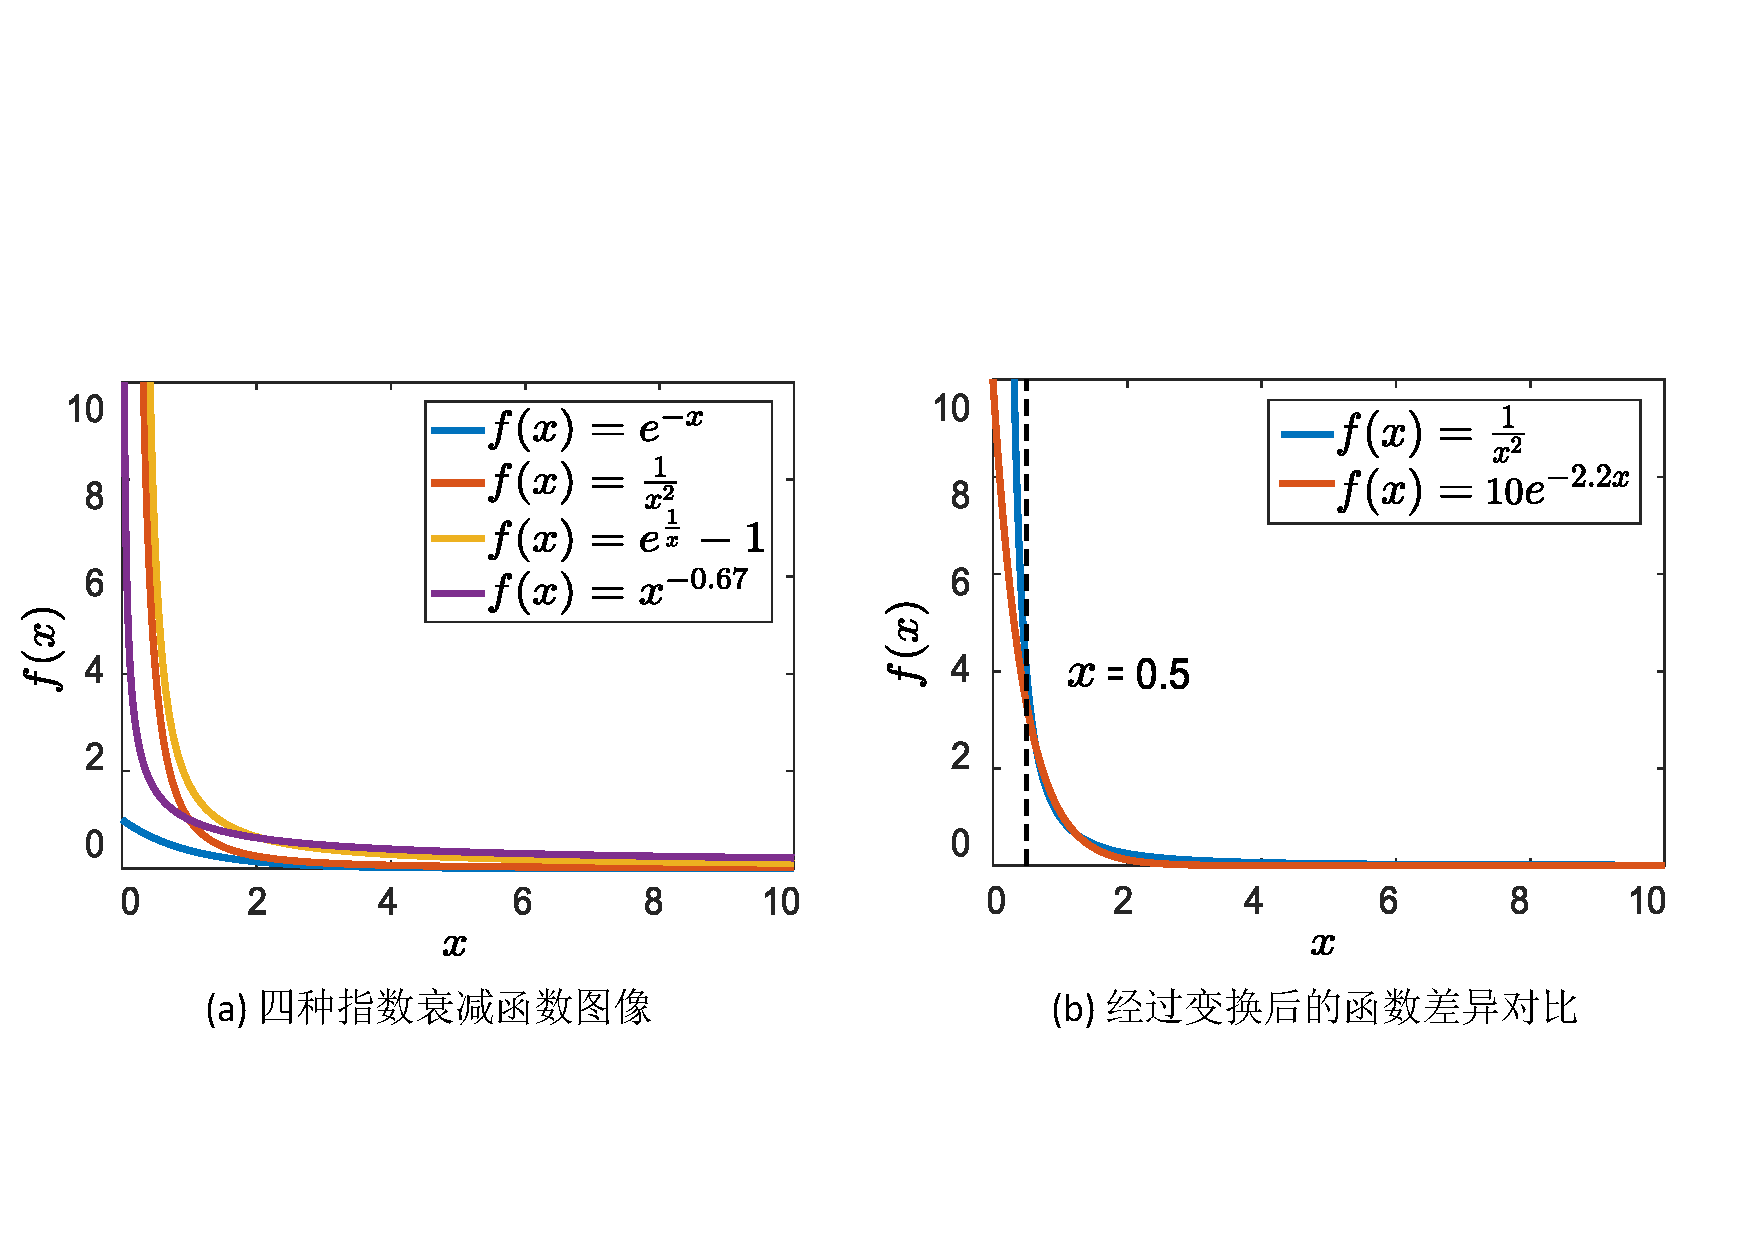
\includegraphics[width=\textwidth]{figure/simplified/simplified_decayfunc v2.pdf}
%\caption[指数衰减函数图像分析]{
%先前工作所用的指数衰减函数图像分析。(a) 四种基本类型的指数衰减函数图像。(b) 将函数$e^{-x}$手动调整为$10e^{-2.2x}$,使其图像在区间$(0.5, +\infty)$内与函数$\frac{1}{x^2}$更接近。}
\caption[指数衰减函数图像变换与差异分析]{
指数衰减函数图像变换与差异分析
}
\label{fig:simplified_decayfunc}
\end{figure}


\section{简化的社会力模型}

\subsection{智能体受力分析与基类设计}
\label{section:simplified_basicclass}

基于上一章节的分析,我们提出了一种只使用简化的单一函数模型去描述所有仿真过程中涉及到的社会力,避免对不同的交互行为使用不同的模型进行专门的建模。我们重新定义,对于任意智能体$i$而言,其运动期间所受合力表示为:
\begin{equation}
\setlength\abovedisplayskip{6pt}
\setlength\belowdisplayskip{6pt}
\label{eq:simplified_newtotalforce}
        \textbf{F}_i = \textbf{F}_i^0 + \sum_{j\in{A\cup{W}}(\not=i)}\textbf{F}_{ij}.
\end{equation}
作为表达式~\ref{eq:simplified_previous}的简化,上式右侧的第一项$\textbf{F}_i^0$仍然用于表示智能体$i$的自驱动力,而第二项则用于表示外界对$i$施加的交互力$\textbf{F}_{ij}$的总和,施力方$j$可以是来自智能体集合$A$中的任意类型智能体,也可以是来自环境因素集合$W$中的障碍物或车道线。交互力$\textbf{F}_{ij}$又由两部分组成:
\begin{equation}
\setlength\abovedisplayskip{6pt}
\setlength\belowdisplayskip{6pt}
\label{eq:simplified_simpforce}
        \textbf{F}_{ij} = \textbf{F}_{ij}^D + \textbf{F}_{ij}^T,
\end{equation}
其中$\textbf{F}_{ij}^D$为直接排斥力,表示在运动过程中沿着$j$指向$i$方向的排斥效果以避免$i$过于接近并发生碰撞,$\textbf{F}_{ij}^T$为横向避让力,表示垂直于$i$和$j$连线方向上发生的侧向避让或超越等行为。图~\ref{fig:simplified_forcediagram}展示了部分情况下不同智能体在不同交互场景下的受力情况。值得注意的是,由于车辆始终倾向于保持在车道中心线行驶,所以在确认满足变道条件后,车辆的变道行为可以直接通过车道线对其施加的吸引力实现,而不需要考虑前车施加的横向避让力,如图~\ref{fig:simplified_forcediagram}(c)所示。


\begin{figure}[t]
\centering
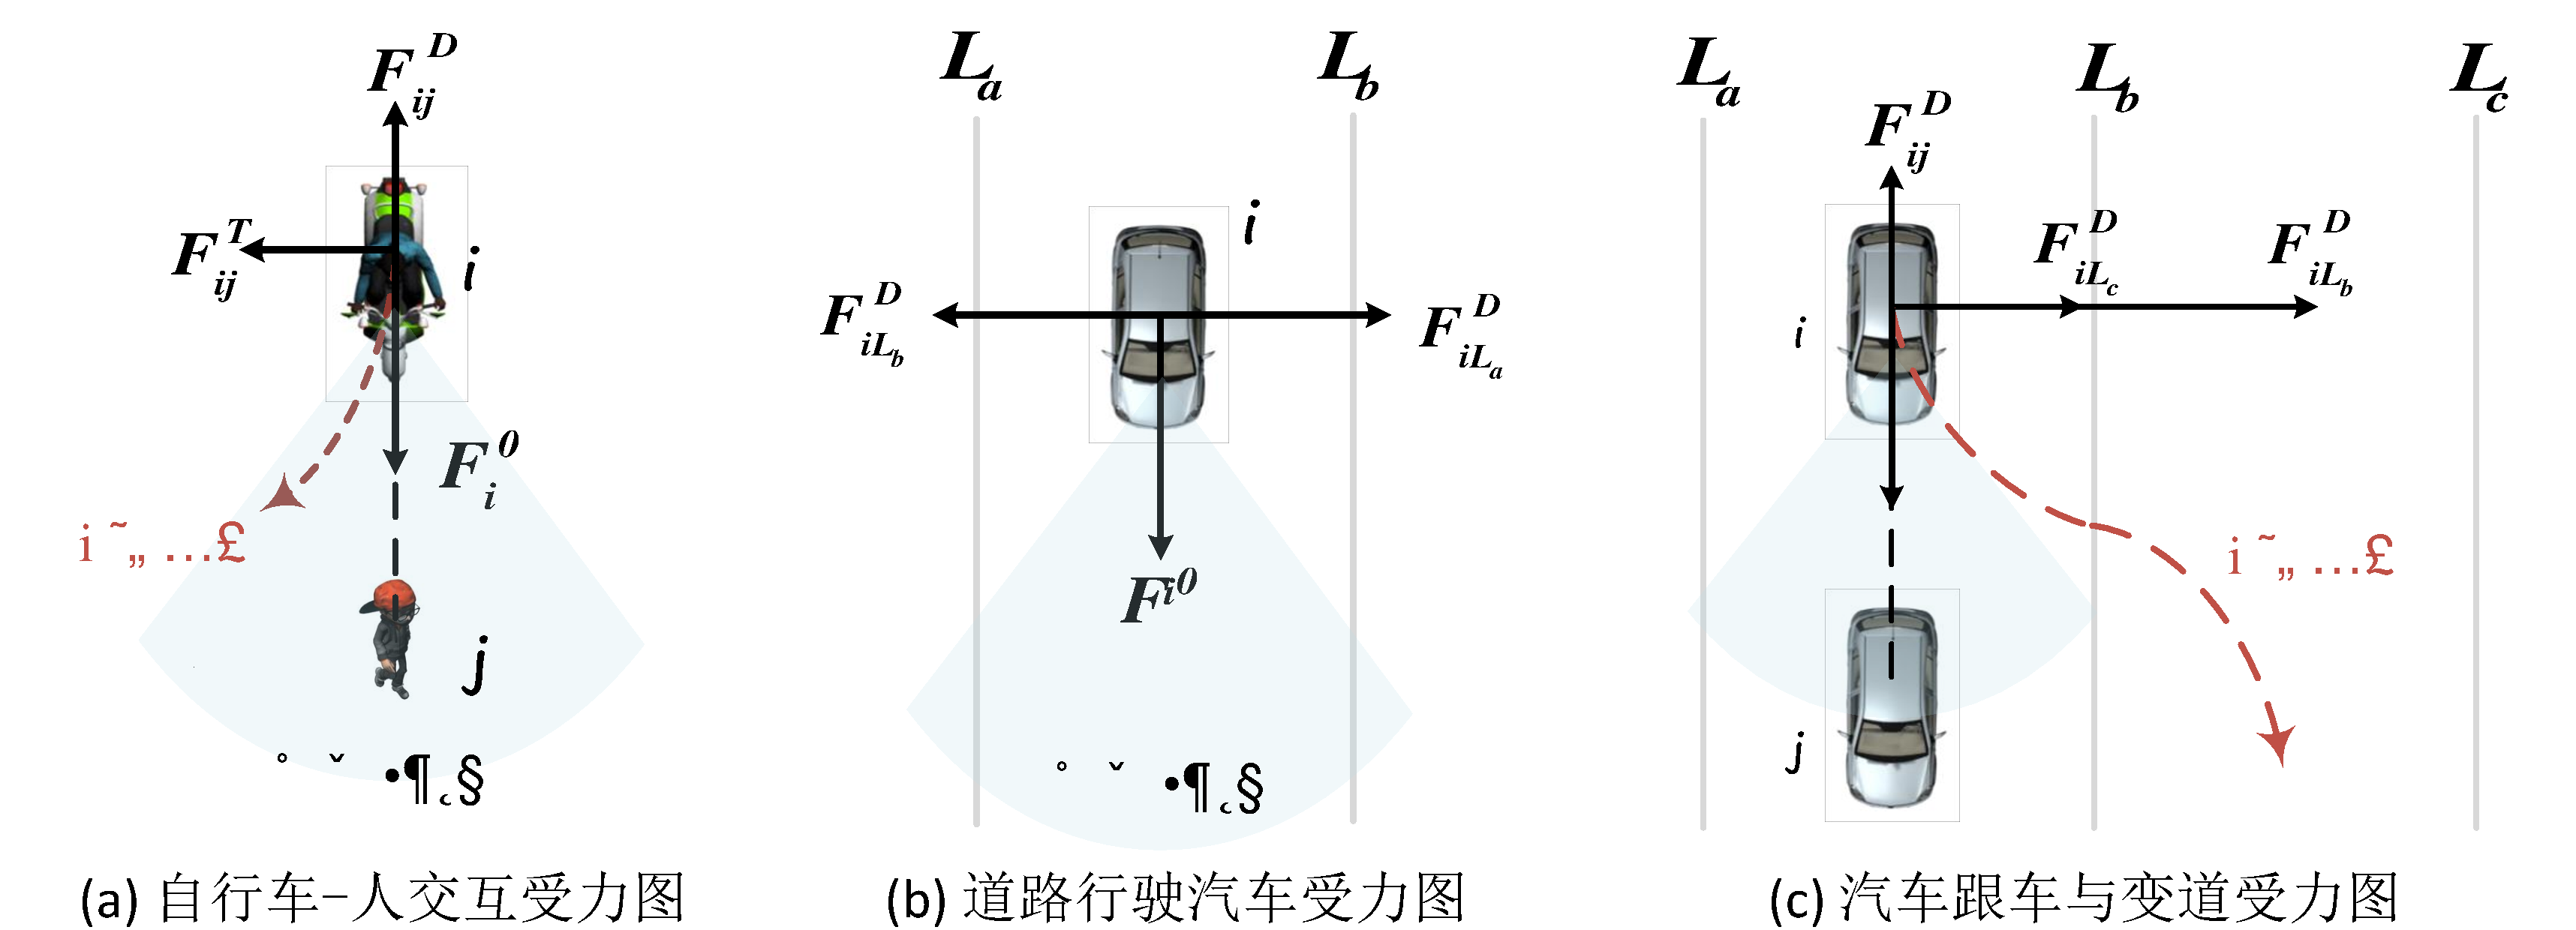
\includegraphics[width=\textwidth]{figure/simplified/simplified_forcediagram_cn_v2.pdf}
%\caption[不同交互场景智能体的受力情况]{
%本方法中不同交互场景下智能体的受力情况。(a) 自行车在与前方的行人交互时的受力情况。(b) 车辆在沿着道路行驶时的受力情况。(c) 车辆在与同车道的前车交互并尝试变道时的受力情况。}
\caption[不同场景中智能体的受力情况]{
不同场景中智能体的受力情况
}
\label{fig:simplified_forcediagram}
\end{figure}

直接排斥力和横向避让力的计算函数模型应该满足以下几个特点:
\begin{itemize}
    \item 函数数值在区间$(0, +\infty)$内平滑缓慢变化;
    \item 当交互对象之间的距离非常大时,计算得到的力应该小到足以被忽视;
    \item 当交互对象之间的距离非常小时,计算得到的力的大小需要能够满足制动或超车的需求,而同时也应该避免趋向于无穷大,导致一个无穷大的力施加在某一智能体上造成其运动的失真。
\end{itemize}

基于这些标准,我们将直接排斥力定义为:
\begin{equation}
\setlength\abovedisplayskip{6pt}
\setlength\belowdisplayskip{6pt}
\label{eq:simplified_directrepulsion}
    \textbf{F}_{ij}^D(d_{ij}) = \left[ \frac{\alpha}{(1 + \beta \cdot d_{ij})^2} + c \right] \textbf{n}_{ij},
\end{equation}
其中$\textbf{n}_{ij}$表示由$j$指向$i$的单位向量,$d_{ij}$表示$i$和$j$之间的距离,$\alpha, \beta$为控制函数趋势的缩放和偏移系数,从而使该模型能够仿真出不同类型智能体的行为。具体来说,系数$\alpha$确定了函数值的最大值,系数$\beta$用于控制函数值对距离$d_{ij}$变化的敏感程度,系数$c$则用于保证函数输出的数值始终非负,在后续实验中由于$\alpha$总是为正因此$c$恒等于0。

受Kesting等人~\cite{kesting2007general}的工作启发,我们将横向排斥力定义为垂直于$i$和$j$连线方向上的力,其数值大小正比于直接排斥力:
\begin{equation}
\setlength\abovedisplayskip{6pt}
\setlength\belowdisplayskip{6pt}
\label{eq:simplified_latealavoidance}
    \textbf{F}_{ij}^T(d_{ij}) = k \| \textbf{F}_{ij}^D(d_{ij}) \| \textbf{n}_{ij}^V,
\end{equation}
其中$\textbf{n}_{ij}^V$是垂直于$\textbf{n}_{ij}$的单位向量,$k$是一个视角系数,在后续实验中设为$i$运动方向和$i$指向$j$方向的夹角的余弦值。

通过上述简化的社会力模型,我们就可以设计出一个能刻画出智能体在交互过程中行为共性的基类,包括点到点方向上的直接避让,与垂直于该方向上的横向避让。但由于不同类型的个体拥有不同的运动学模型,因此具体的行为表现还需要通过重载上述直接排斥力与横向避让力的计算过程,从而派生出行人、车和自行车的多种类智能体。


\subsection{系数参数化与基类派生}
\label{section:simplified_parameterize}

如前文所述,表达式~\ref{eq:simplified_directrepulsion}中定义的系数$\alpha, \beta$是智能体基类派生出不同种类智能体、控制个体具体行为表现的接口。为了达到不同种类智能体行为的差异化和同类智能体不同个体行为的个性化,我们基于个体独有的物理属性来参数化这些系数,让每个个体都能根据自己的情况来采取相应的行为。参数化的过程定义为:
\begin{equation}
\setlength\abovedisplayskip{6pt}
\setlength\belowdisplayskip{6pt}
\label{eq:simplified_parameterize}
    \left\{
        \begin{array}{lr}
        \alpha = s_{i0} + \|v_i\| T_i + \frac{\|v_i\| \|\Delta v_{ij}\|}{2\sqrt{a_i b_i}}, & \\
        \beta = \frac{1}{s_{i0}},
        \end{array}
    \right.
\end{equation}
其所涉及的参数$(s_{i0}, v_i, T_i, \Delta v_{ij}, a_i, b_i)$中,$s_{i0}$表示智能体$i$的期望与其他个体保持的安全距离,$v_i$表示$i$的当前时刻下的速度,$T_i$表示$i$采取制动行为所需要的反应时间,$\Delta v_{ij}$表示$i$和$j$之间在当前时刻下的相对速度,$a_i, b_i$表示$i$的最大加速度和最大减速度。


由于不同个体上述的参数预设各不相同,因此我们使用表达式~\ref{eq:simplified_parameterize}对基类中的力计算过程进行重载,从而得到不同种类智能体、同种类智能体不同表现细节的交互行为。表~\ref{tab:simplified_pvalues}总结了在实验过程中不同种类智能体参数的取值范围。由于智能体可能会同时受到多个外力的影响,因此为了防止作用在某一个个体上的合力过大,我们将合力限制在一个正比于其自驱动力数值大小的上限内,以防止智能体运动失真。值得注意的是,与Chao等人的工作~\cite{chao2019force}相比,用户使用我们的仿真方法能够避免调试大量没有实际意义的参数,只需要更改智能体的物理属性就能够与行为的变化产生直观的联系。

\begin{table}[!htb]
%\setlength{\abovecaptionskip}{-0.15cm}
\setlength{\belowcaptionskip}{0.4cm}
\begin{center}
%\caption[实验中不同种类智能体的参数取值范围]{实验中不同种类智能体的参数取值范围。}
\caption[实验中不同种类智能体的参数取值]{实验中不同种类智能体的参数取值}
\label{tab:simplified_pvalues}
\renewcommand\arraystretch{1.2}
\begin{tabular}{|c|ccc|c|c|}
\hline
\multirow{2}{*}{\textbf{参数}} & \multicolumn{3}{c|}{\textbf{取值范围}} & \multirow{2}{*}{\textbf{单位}} & \multirow{2}{*}{\textbf{描述}} \\ \cline{2-4}
 & \multicolumn{1}{c|}{车} & \multicolumn{1}{c|}{自行车} & \multicolumn{1}{c|}{行人} &  &  \\ \hline
$v_i$ & \multicolumn{1}{c|}{[0, 15]} & \multicolumn{1}{c|}{[0, 8]} & [0, 2] & $m/s$ & 实时速度 \\ \hline
$a_i$ & \multicolumn{1}{c|}{[3, 5]} & \multicolumn{1}{c|}{[2, 3]} & [0.5, 1] & $m/s^2$ & 最大加速度 \\ \hline
$b_i$ & \multicolumn{1}{c|}{[3, 5]} & \multicolumn{1}{c|}{[2, 3]} & [0.5, 1] & $m/s^2$ & 最大减速度 \\ \hline
$s_{i0}$ & \multicolumn{1}{c|}{[3, 5]} & \multicolumn{1}{c|}{[1, 3]} & [0.5, 3] & $m$ & 期望与其他个体保持的安全距离 \\ \hline
$T_i$ & \multicolumn{1}{c|}{[0.5, 1]} & \multicolumn{1}{c|}{[0.5, 2]} & [0.5, 2] & $s$ & 制动所需反应时间 \\ \hline
\end{tabular}
\end{center}{}
\end{table}


\section{实验结果}

实验所用的测试场景为一条没有信号灯控制的笔直道路,最中间为双向的机动车道,两侧依次为非机动车道和人行横道,且在整条道路的中间部位设置有一段斑马线供行人穿行。实验所用设备为一台笔记本电脑,配备了8核的2.60GHz Intel(R) Core(TM) i7-4720HQ处理器以及8GB的内存。仿真实验代码均基于CSharp脚本实现,并直接在Unity3D中进行可视化。图~\ref{fig:simplified_snapshot2}展示了一些从俯视或驾驶员位等不同视角观察的,包含行人、车、自行车交互行为的混合交通仿真结果。

\begin{figure}[tbh]
\centering
%\setlength{\abovecaptionskip}{0.1cm}
%\setlength{\belowcaptionskip}{0.25cm}
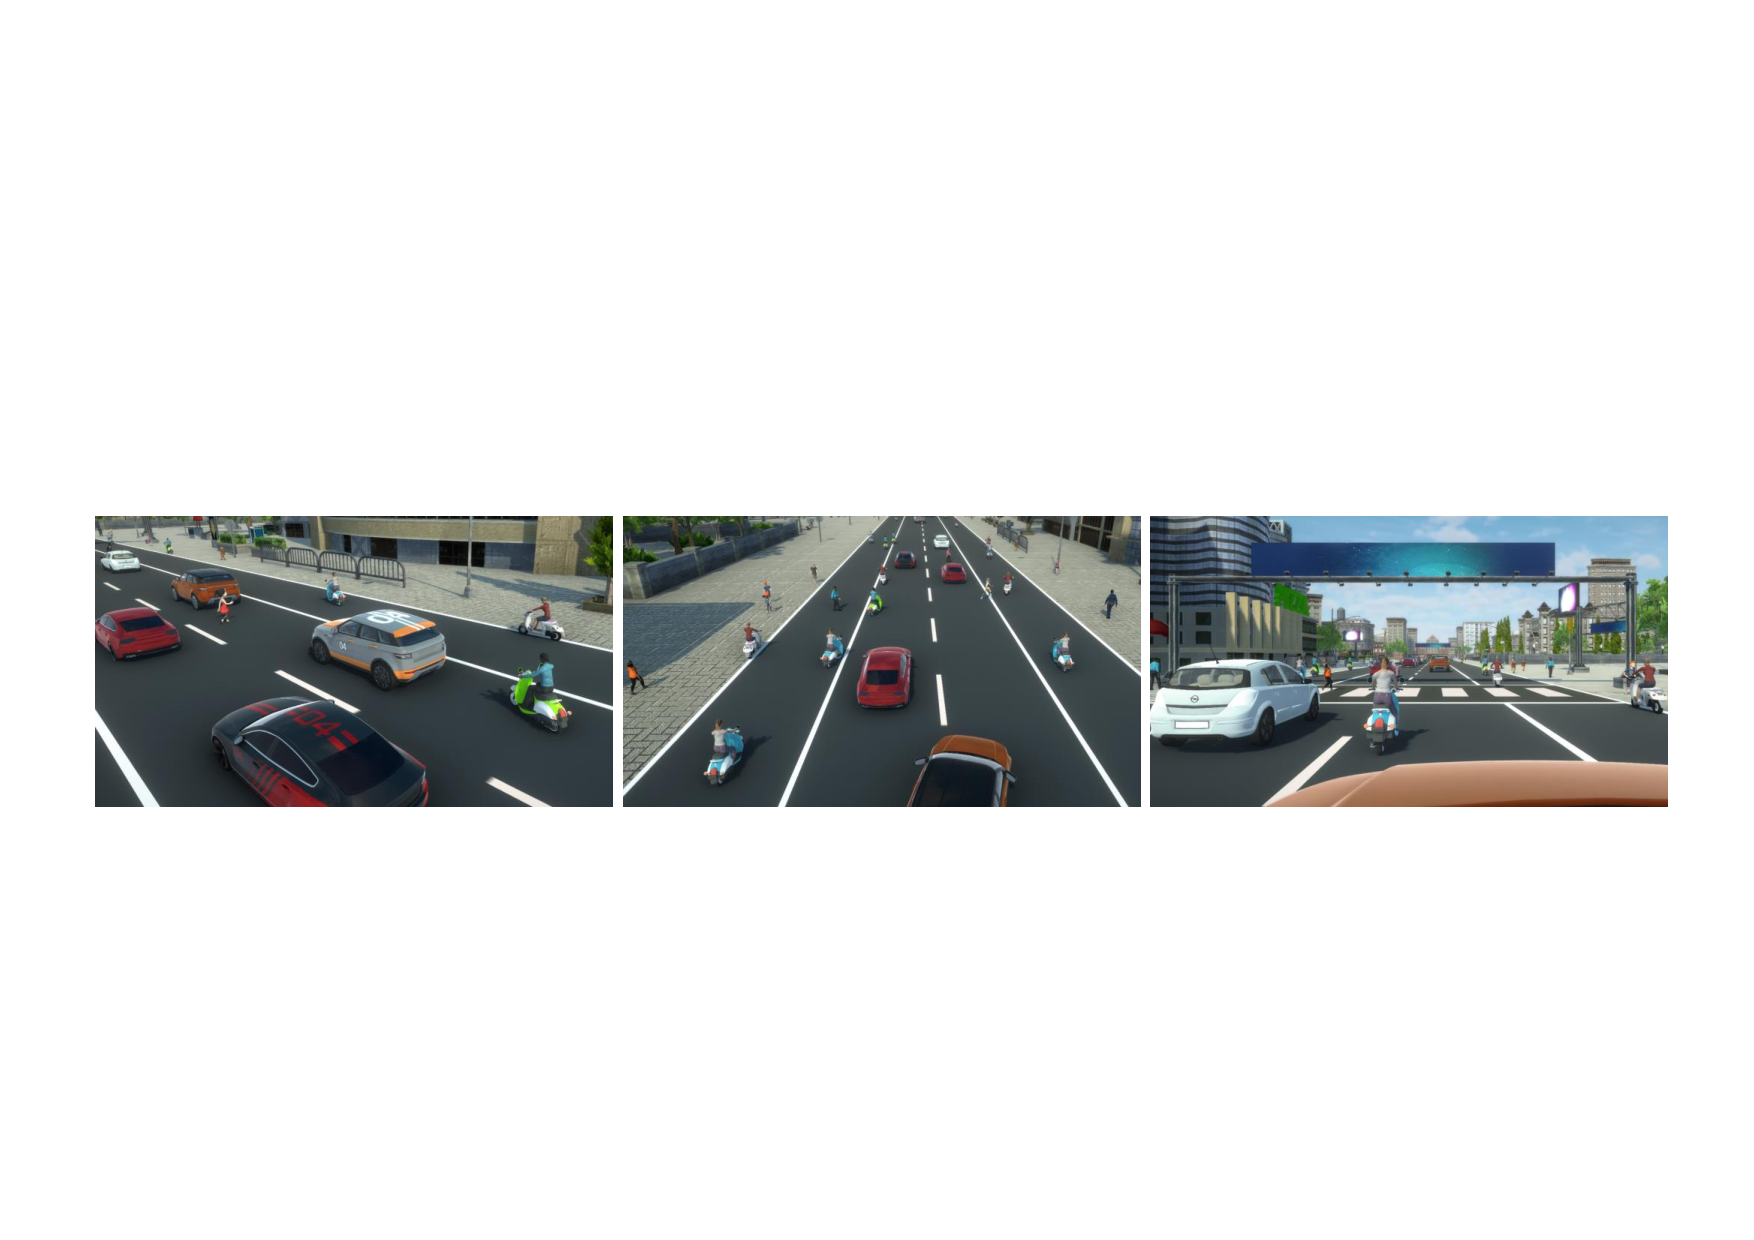
\includegraphics[width=\textwidth]{figure/simplified/simplified_snapshot}
%\caption[不同视角下的多种类智能体交互行为]{
%一些基于本方法仿真,从俯视或驾驶员位等不同视角观察的混合交通仿真结果,包含行人、车、自行车的交互行为。}
\caption[不同视角下的多种类智能体交互行为]{
不同视角下的多种类智能体交互行为
}
\label{fig:simplified_snapshot2}
\end{figure}


\subsection{智能体交互案例}
\label{section:simplified_interactioncase}

\textbf{车-行人交互行为:}如图~\ref{fig:simplified_case1}(a)所示,我们展示了在行人横过马路的场景下,行驶中的车辆与行人交互的行为结果;在图~\ref{fig:simplified_case1}(b)中,我们展示了交互双方最终的轨迹示意图以及分别在沿着运动方向与垂直运动方向上的速度曲线变化。经过观察图片我们发现,车辆在靠近有行人穿行的斑马线时,双方均尝试过减速以等待对方,一段时间后行人决定恢复原始的速度先行通过交互区域,此时车辆速度几乎处于完全制动的状态,而在行人远离后车辆也加速通过了斑马线。此外,我们还注意到行人在横向方向上也发生了位置偏移,这与现实生活中行人过斑马线时存在的横向避让来车行为一致。

\begin{figure}[!tbh]
\centering
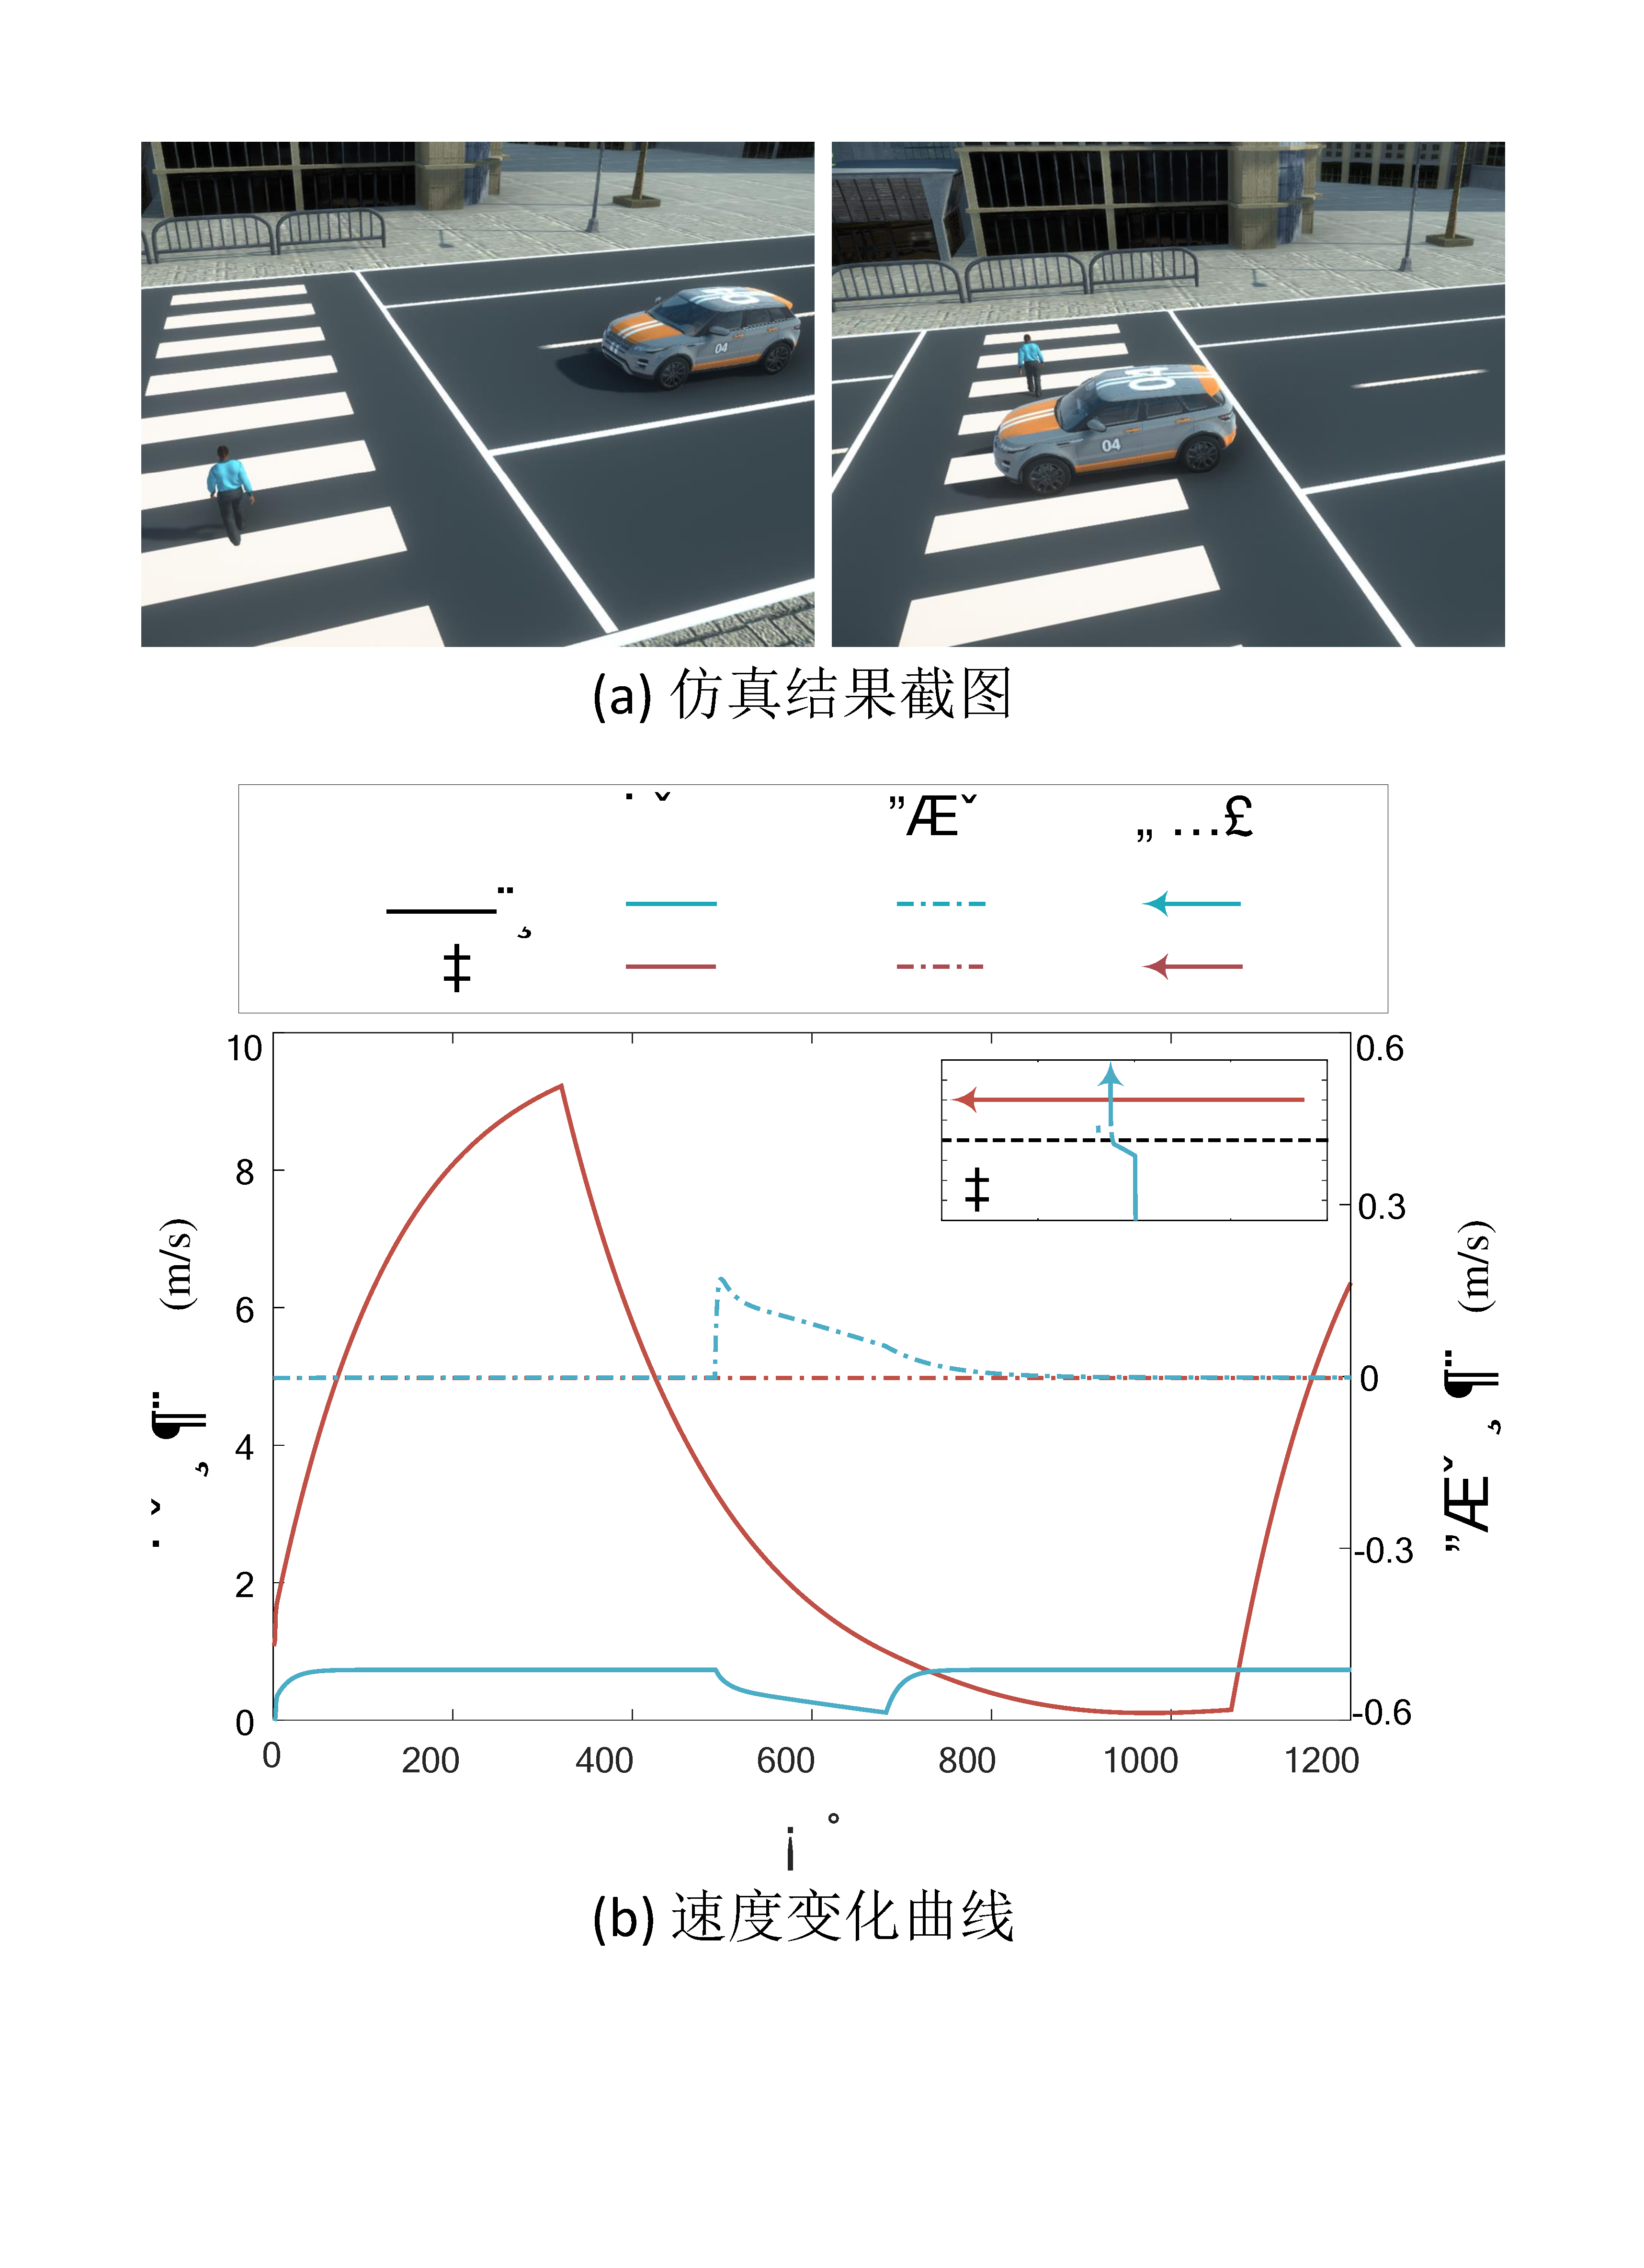
\includegraphics[width=0.58\textwidth]{figure/simplified/simplified_case1_vert_cn v2.pdf}
%\caption[车-行人交互结果与速度曲线]{在行人过马路的场景中,车-行人交互行为的:(a) 仿真结果,(b) 轨迹示意图与速度曲线变化对比。}
\caption[车-行人交互结果与速度曲线]{车-行人交互结果与速度曲线}
\label{fig:simplified_case1}
\end{figure}

\textbf{车辆变道行为:}如图~\ref{fig:simplified_case2}(a)所示,我们展示了在被同车道的低速前车堵塞时,后车展示的变道行为结果;同样地,在图~\ref{fig:simplified_case2}(b)中我们展示了交互双方的最终轨迹示意图以及分别在沿着运动方向与垂直运动方向上的速度曲线变化。经过观察我们发现,后车在靠近低速前车的过程中其首先尝试直接减速以避免碰撞,随后在邻车道无其他车辆和障碍物且前车持续保持低速运行的情况下,后车决定向左变道以绕过前车,最终恢复原始速度实现了超车。

\begin{figure}[!tbh]
\centering
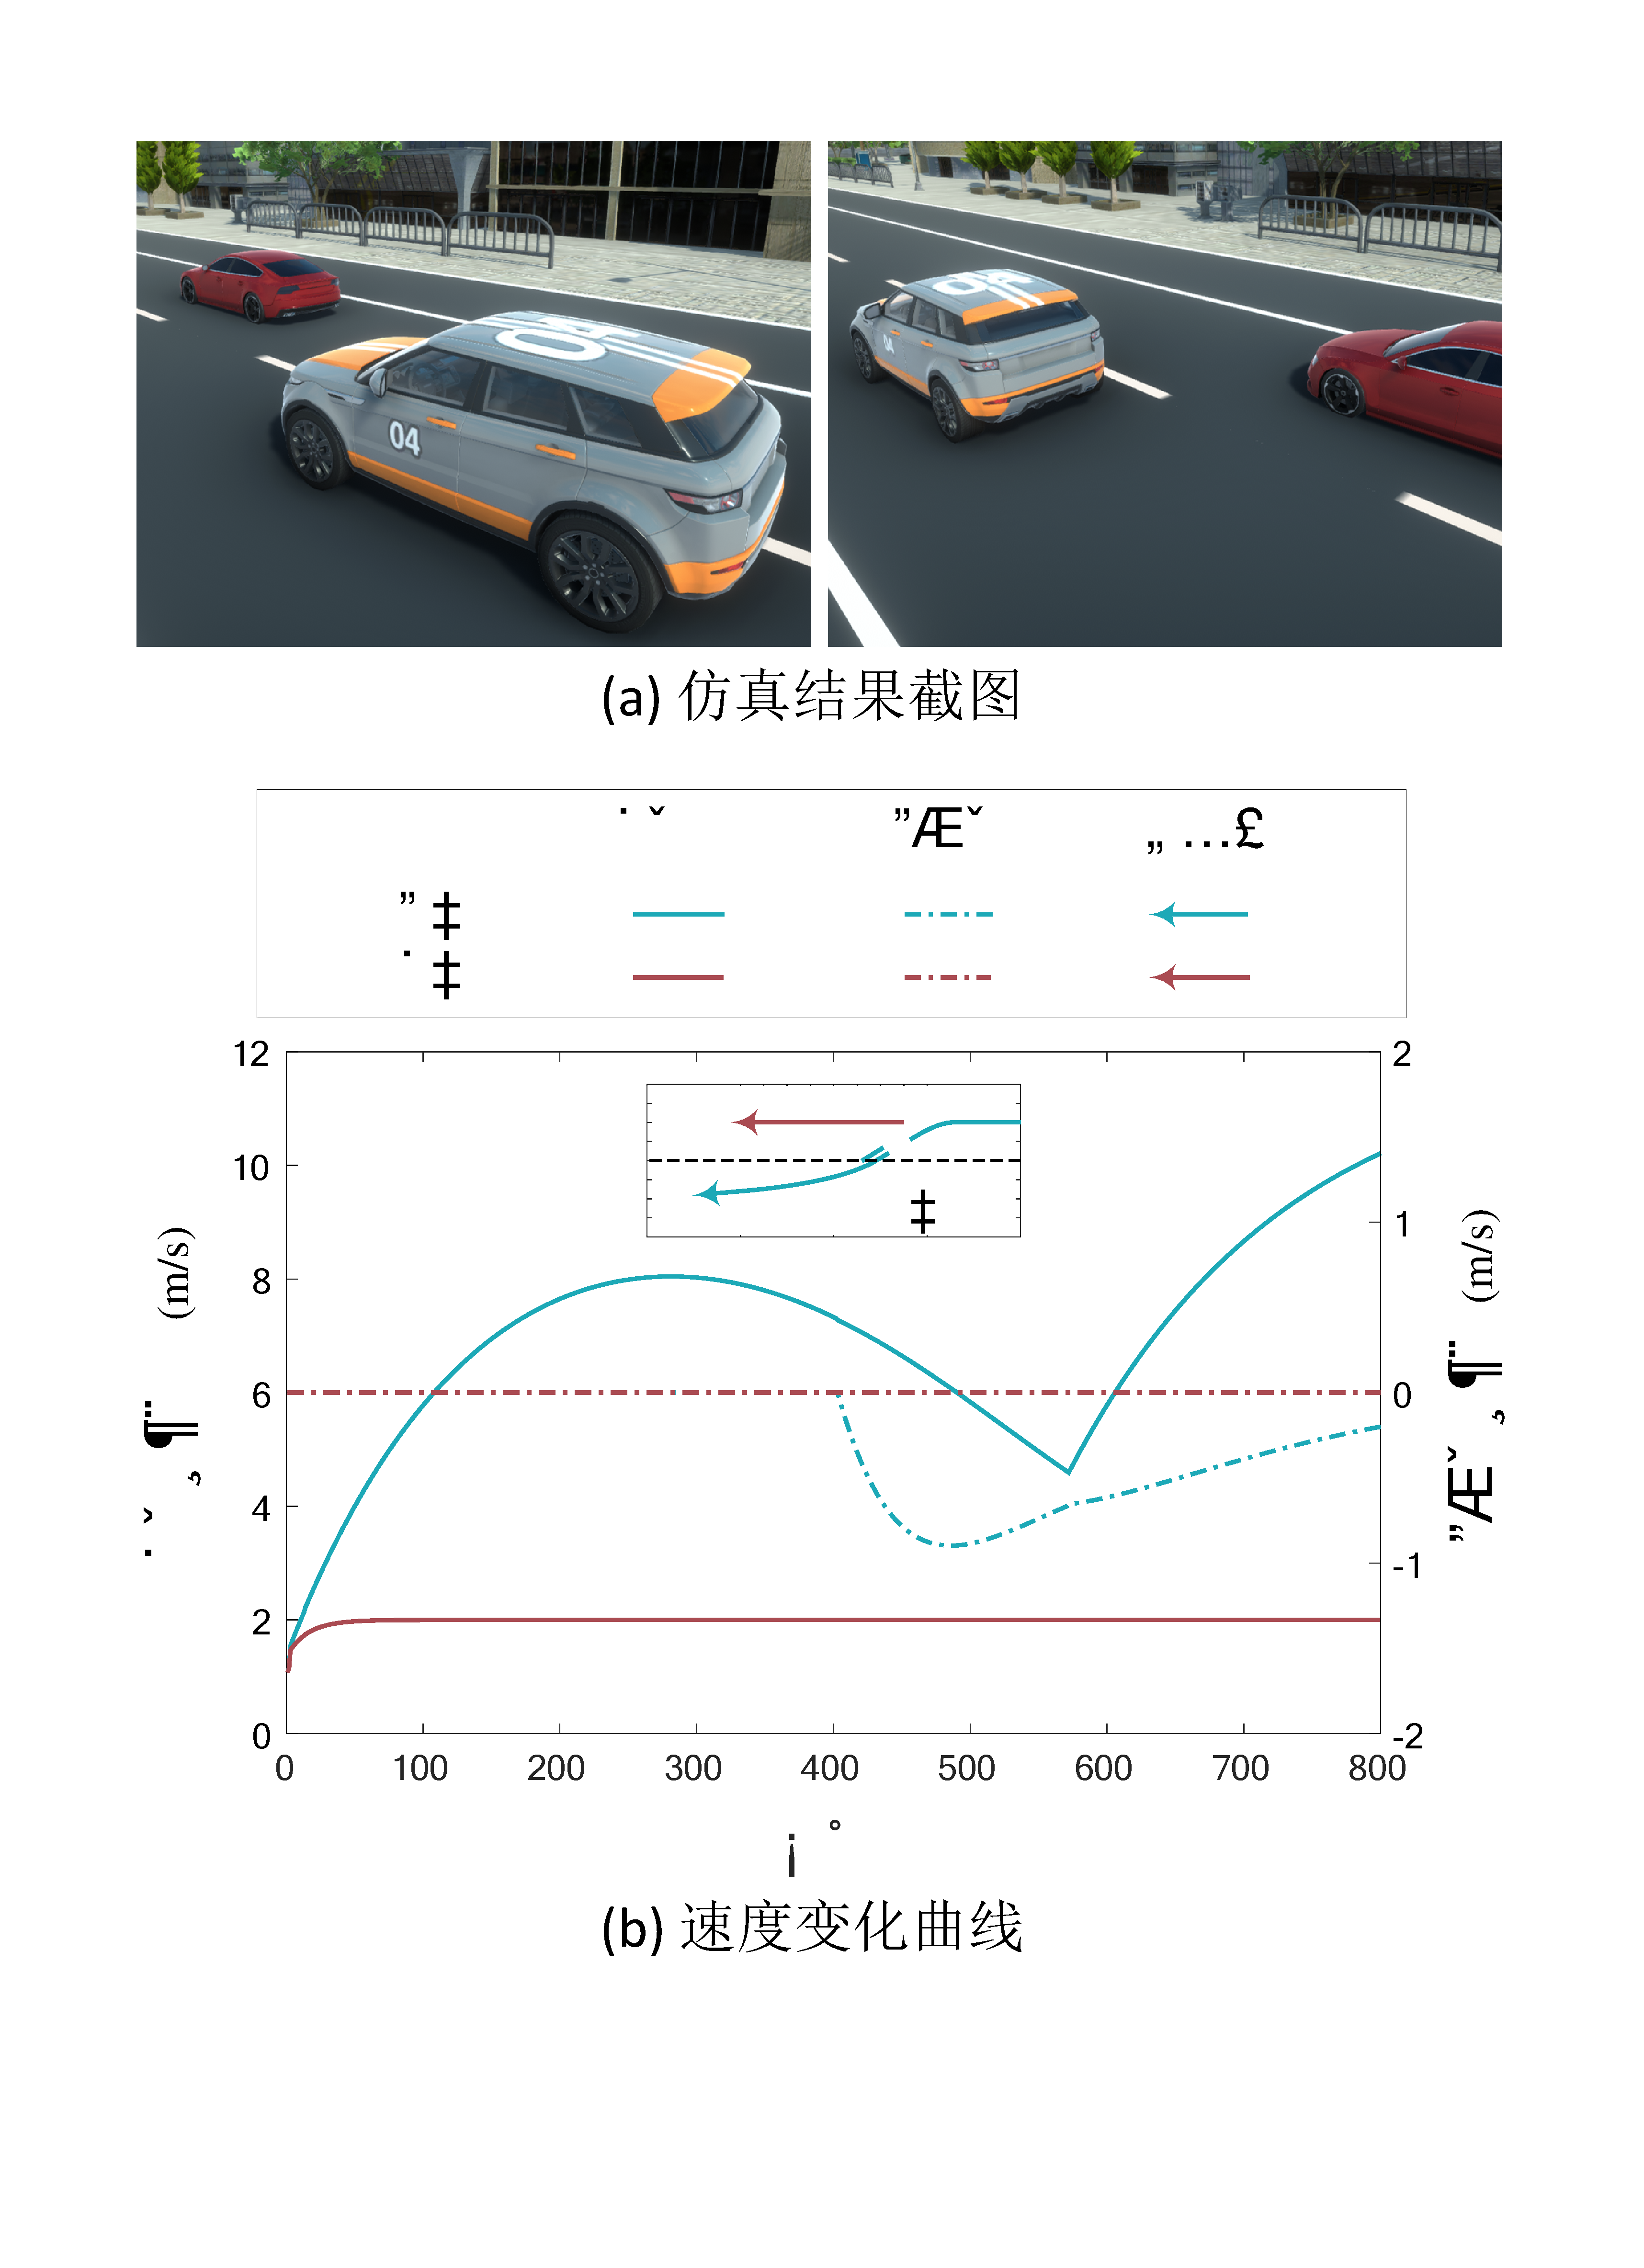
\includegraphics[width=0.58\textwidth]{figure/simplified/simplified_case2_vert_cn v2.pdf}
%\caption[车辆变道结果与速度曲线]{在同车道两车跟车行驶的场景中,后车变道行为的:(a) 仿真结果,(b) 轨迹示意图与速度曲线变化对比。}
\caption[车辆变道结果与速度曲线]{
车辆变道结果与速度曲线
}
\label{fig:simplified_case2}
\end{figure}

\textbf{车-自行车交互行为:}如图~\ref{fig:simplified_case3}(a)所示,我们还展示了在自行车突然从非机动车车道冲入机动车道时,后方来车与自行车的交互行为结果;同样地,在图~\ref{fig:simplified_case3}(b)中我们展示了对应行为的交互双方的轨迹示意图与分别在沿着运动方向和垂直运动方向上的速度曲线变化。经过观察我们发现,当自行车突然冲入机动车道时,后方车辆有一个突然的急刹车行为以迅速降低行驶速度,并且在横向上有一个向右避让的行为,而在自行车稳定且回到非机动车道上之后,车辆除了恢复到原始的速度外还回到了车道中心行驶,这也与现实世界中驾驶员在紧急情况下采取的避让措施一致。

\begin{figure}[!tbh]
\centering
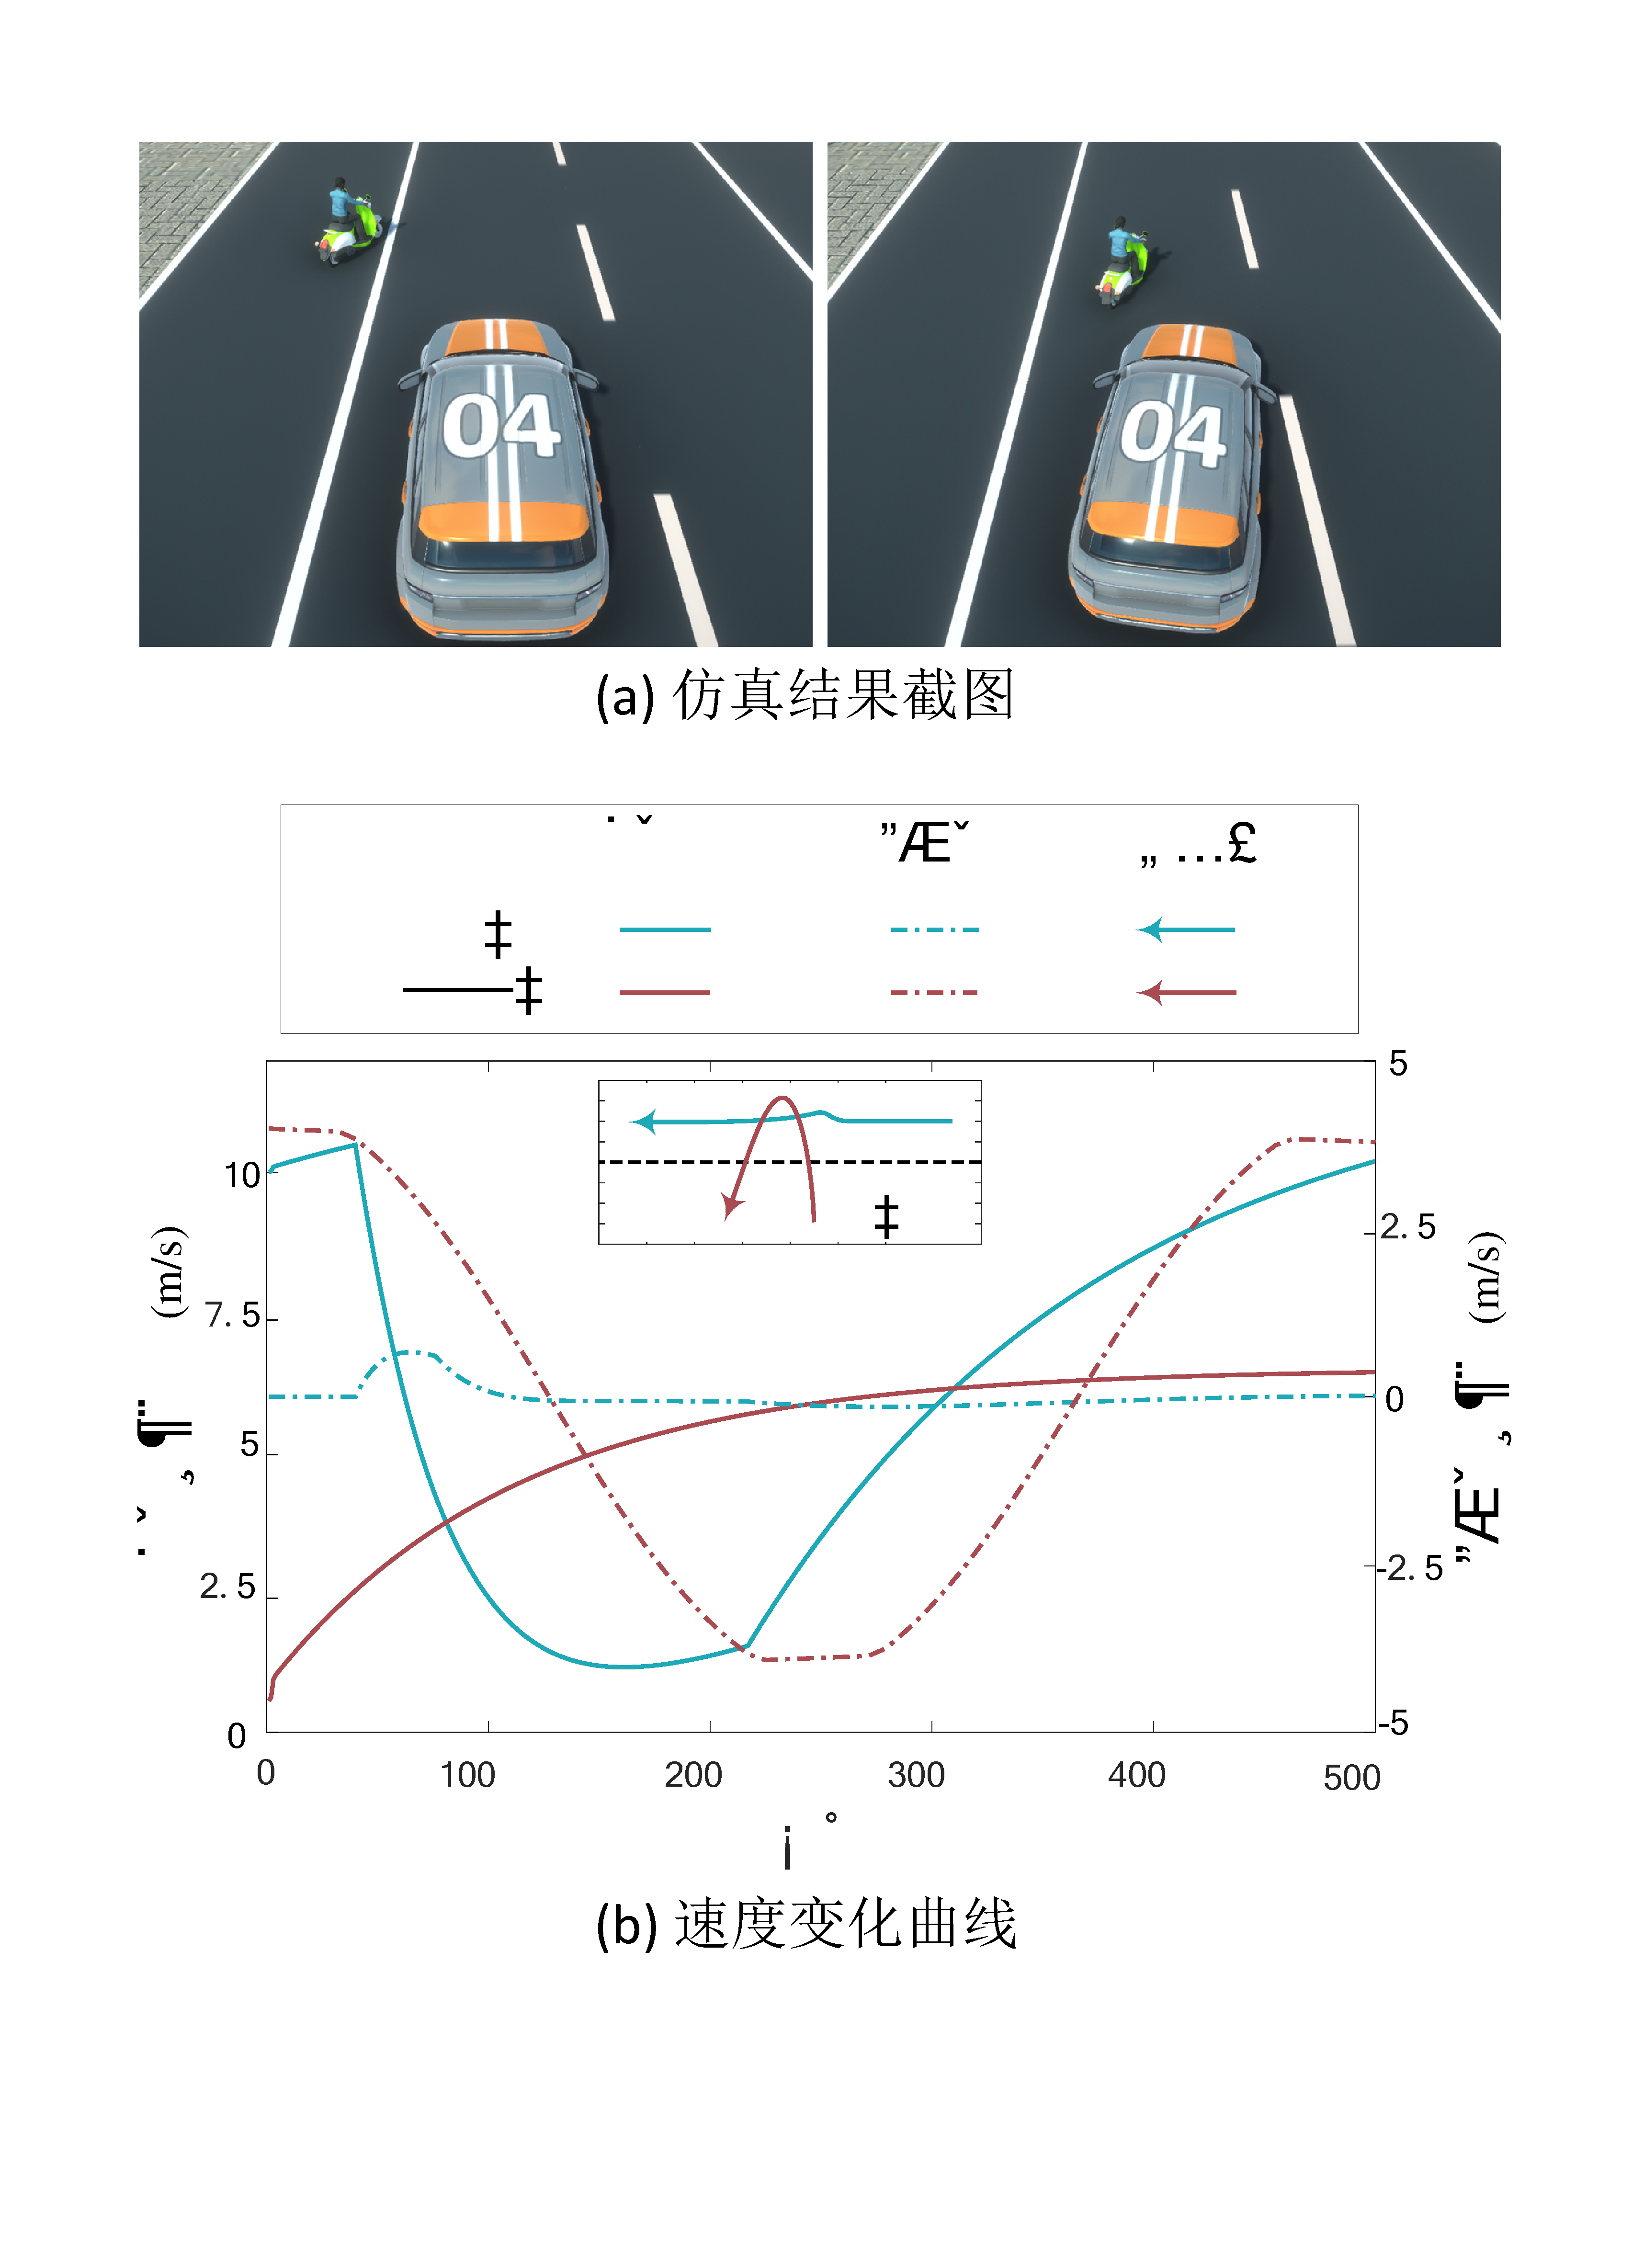
\includegraphics[width=0.58\textwidth]{figure/simplified/simplified_case3_vert_cn v2.pdf}
%\caption[车-自行车交互结果与速度曲线]{在自行车突然从非机动车道冲入机动车道,车-自行车交互行为的:(a) 仿真结果,(b) 轨迹示意图与速度曲线变化对比。}
\caption[车-自行车交互结果与速度曲线]{
车-自行车交互结果与速度曲线
}
\label{fig:simplified_case3}
\end{figure}


\subsection{性能分析}
\label{section:simplified_performance}

我们通过在场景中放置不同数量的智能体以测试我们的方法的计算效率,其中车、自行车、行人的数量比例保持为$1:2:3$。在上述一系列实验过程中,我们只保留了车道路面模型而将其他场景物体省去,且使用简单的白模几何体来代替智能体,从减少因数据加载,渲染或其他仿真无关的操作引起的时间消耗。图~\ref{fig:simplified_performance}(a)展示了我们的方法在不同数量智能体场景中每一帧的仿真耗时,以及每一帧调用力计算模型的次数。经过观察我们发现,每一帧的仿真计算的时间和力计算模型的调用次数均随着智能体数量的增加几乎呈线性增长,二者的趋势几乎相同,且智能体数量在1400左右时仍然能够保持30fps的计算帧率。

考虑到本方法是基于Chao等人工作~\cite{chao2019force}的一个优化,我们还设计了一个特别的对比实验。同样是在一个与3D场景加载和渲染无关的环境下,我们调用若干次Chao等人的力计算模型与我们提出的简化的社会力模型,在保持调用次数相同的情况下,我们比较调用不同模型最终的计算耗时。这个任务旨在证明我们提出的简化的社会力模型在大规模的仿真场景中,模型本身的计算用时并不会成为运行效率上的负担(如在成千上万人的体育场或演唱会中,需要大量调用力计算模型计算交互行为)。结果如图~\ref{fig:simplified_performance}(b)所示,由于我们的简化社会力模型基于反比例函数设计,因此在调用次数达到$10^5$量级时仍然保持着出色的计算效率;而Chao等人的工作中使用的力计算模型包含了大量指数计算,导致其将会随着仿真规模的变大最终变得非常耗时。


\begin{figure}[tbh]
\centering
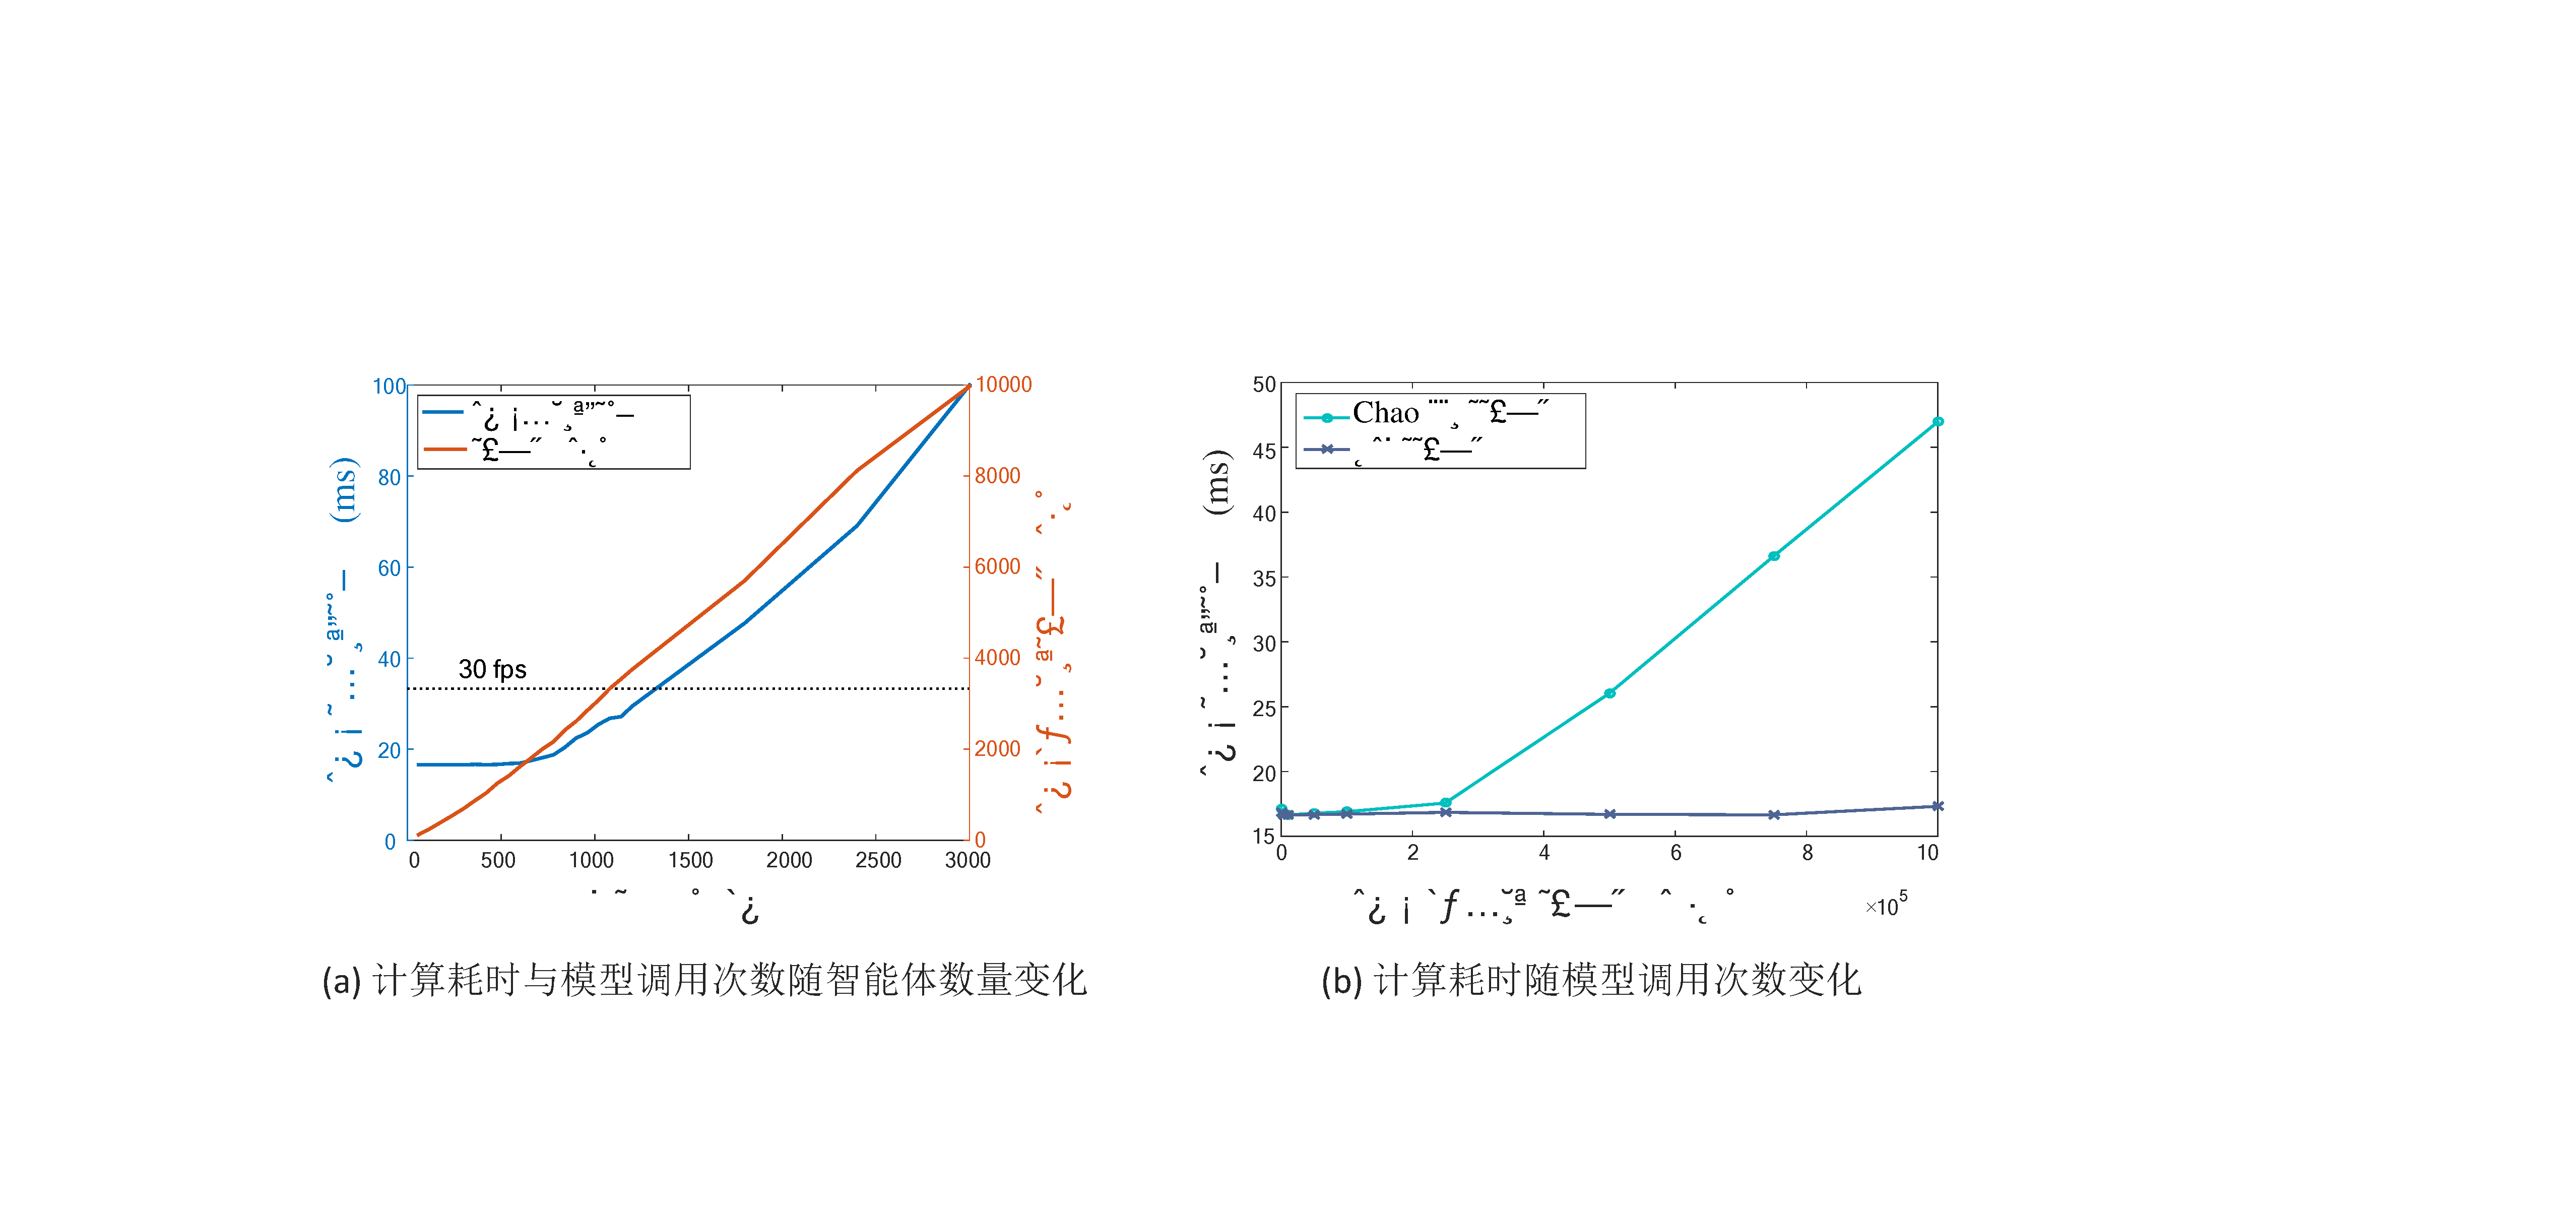
\includegraphics[width=\textwidth]{figure/simplified/simplified_perform_cn_v2.pdf}
%\caption[基于简化社会力模型的混合交通仿真性能分析与对比]{
%本方法的计算效率实验。(a) 本方法在不同数量智能体的场景中,每一帧的的平均计算时间与力计算模型调用次数。(b) 本方法的计算时间与Chao等人方法~\cite{chao2019force}的对比结果。}
\caption[本方法的性能统计与对比]{
本方法的性能统计与对比
}
\label{fig:simplified_performance}
\end{figure}


\section{本章小结}

本章工作提出了一个基于简化的社会力模型的混合交通仿真方法,用于仿真包含行人、车、自行车等多种类智能体交互行为的场景,以提升可视化交通仿真中仿真个体的种类多样性。基于面向对象的思想,我们设计了一个能描述智能体行为共性的基类,并使用简化的社会力模型来表达和计算智能体之间交互,包括沿着点对点连线方向的直接排斥力和垂直于该方向的横向避免力。通过使用每个个体独有的物理属性,我们将简化的社会力模型中的无物理意义的系数参数化,把基类派生出不同种类的智能体,且拥有各自不同的行为模式。本方法的混合交通仿真框架更简洁,更易扩展,且具有更高的计算效率,能够快捷地作为插件集成到现有的仿真平台如百度Apollo或Carla,用于自动驾驶的测试。

本方法在以下几个方向仍具有继续研究的价值。其一,本方法可以使用真实的交通轨迹数据进行标定而不是凭经验地进行设置,从而为每个个体的物理属性和模型参数选择更适当的取值,生成更真实的仿真结果。其二,在模型系数参数化的建模中可以考虑更多样的因素,例如运动学约束、群体密度、道路的最大限速或者是个体对不同类型交互对象的反应敏感度。具体来说,个体通常对不同类型的智能体会采取不同的反应行为,如行人通常会觉得车辆比自行车更具有威胁,因此会更早采取避让措施以远离危险。其三,本方法当前基于纯数理建模,我们亦可引入更多的基于学习的策略,最大化利用真实交通轨迹数据对个体受力或系数参数化进行模糊建模。

